%%%%%%%%%%%%%%%%%%%%%%%%%%%%%%%%%%%%%%%%%%%%%%%%%%%%%%%%%%%%%%%%
%
% Apuntes de la asignatura Análisis Matemático II.
% Doble Grado de Informática y Matemáticas.
% Universidad de Granada.
% Curso 2016/17.
% 
% 
% Colaboradores:
% Javier Sáez (@fjsaezm)
% Daniel Pozo (@danipozodg)
% Pedro Bonilla (@pedrobn23)
% Guillermo Galindo
% Antonio Coín (@antcc)
% Sofía Almeida (@SofiaAlmeida)
% Miguel Lentisco (@AlfaOmegaX)
%
% Agradecimientos:
% Andrés Herrera (@andreshp) y Mario Román (@M42) por
% las plantillas base.
%
% Sitio original:
% https://github.com/libreim/apuntesDGIIM/
%
% Licencia:
% CC BY-NC-SA 4.0 (https://creativecommons.org/licenses/by-nc-sa/4.0/)
%
%%%%%%%%%%%%%%%%%%%%%%%%%%%%%%%%%%%%%%%%%%%%%%%%%%%%%%%%%%%%%%%


%------------------------------------------------------------------------------
%   ACKNOWLEDGMENTS
%------------------------------------------------------------------------------

%%%%%%%%%%%%%%%%%%%%%%%%%%%%%%%%%%%%%%%%%%%%%%%%%%%%%%%%%%%%%%%%%%%%%%%%
% Plantilla básica de Latex en Español.
%
% Autor: Andrés Herrera Poyatos (https://github.com/andreshp) 
%
% Es una plantilla básica para redactar documentos. Utiliza el paquete  fancyhdr para darle un
% estilo moderno pero serio.
%
% La plantilla se encuentra adaptada al español.
%
%%%%%%%%%%%%%%%%%%%%%%%%%%%%%%%%%%%%%%%%%%%%%%%%%%%%%%%%%%%%%%%%%%%%%%%%%

%%%
% Plantilla de Trabajo
% Modificación de una plantilla de Latex de Frits Wenneker para adaptarla 
% al castellano y a las necesidades de escribir informática y matemáticas.
%
% Editada por: Mario Román
%
% License:
% CC BY-NC-SA 3.0 (http://creativecommons.org/licenses/by-nc-sa/3.0/)
%%%

%%%%%%%%%%%%%%%%%%%%%%%%%%%%%%%%%%%%%%%%
% Short Sectioned Assignment
% LaTeX Template
% Version 1.0 (5/5/12)
%
% This template has been downloaded from:
% http://www.LaTeXTemplates.com
%
% Original author:
% Frits Wenneker (http://www.howtotex.com)
%
% License:
% CC BY-NC-SA 3.0 (http://creativecommons.org/licenses/by-nc-sa/3.0/)
%
%%%%%%%%%%%%%%%%%%%%%%%%%%%%%%%%%%%%%%%%%


% Tipo de documento y opciones.
\documentclass[11pt, a4paper, titlepage]{article}


%---------------------------------------------------------------------------
%   PAQUETES
%---------------------------------------------------------------------------

% Idioma y codificación para Español.
\usepackage[utf8]{inputenc}
\usepackage[spanish, es-tabla, es-lcroman, es-noquoting]{babel}
\selectlanguage{spanish} 
%\usepackage[T1]{fontenc}

% Fuente utilizada.
\usepackage{courier}    % Fuente Courier.
\usepackage{microtype}  % Mejora la letra final de cara al lector.

% Diseño de página.
\usepackage{fancyhdr}   % Utilizado para hacer títulos propios.
\usepackage{lastpage}   % Referencia a la última página.
\usepackage{extramarks} % Marcas extras. Utilizado en pie de página y cabecera.
\usepackage[parfill]{parskip}    % Crea una nueva línea entre párrafos.
\usepackage{geometry}            % Geometría de las páginas.

% Símbolos y matemáticas.
\usepackage{amssymb, amsmath, amsthm, amsfonts, amscd}
\usepackage{upgreek}

% Otros.
\usepackage{enumitem}   % Listas mejoradas.
\usepackage[hidelinks]{hyperref}
\usepackage{graphicx}   % Gráficos.


%---------------------------------------------------------------------------
%   OPCIONES PERSONALIZADAS
%---------------------------------------------------------------------------

% Redefinir letra griega épsilon.
\let\epsilon\upvarepsilon

% Formato de texto.
\linespread{1.1}            % Espaciado entre líneas.
\setlength\parindent{0pt}   % No indentar el texto por defecto.
\setlist{leftmargin=.5in}   % Indentación para las listas.

% Estilo de página.
\pagestyle{fancy}
\fancyhf{}
\geometry{left=3cm,right=3cm,top=3cm,bottom=3cm,headheight=1cm,headsep=0.5cm}   % Márgenes y cabecera.

% Redefinir entorno de demostración (reducir espacio superior)
%\makeatletter
%\renewenvironment{proof}[1][\proofname] {\vspace{-15pt}\par\pushQED{\qed}\normalfont\topsep6\p@\@plus6\p@\relax\trivlist\item[\hskip\labelsep\it#1\@addpunct{.}]\ignorespaces}{\popQED\endtrivlist\@endpefalse}
%\makeatother

% Aumentar el tamaño del interlineado
\linespread{1.3}
%---------------------------------------------------------------------------
%   COMANDOS PERSONALIZADOS
%---------------------------------------------------------------------------

% Valor absoluto: \abs{}
\providecommand{\abs}[1]{\lvert#1\rvert}    

% Fracción grande: \ddfrac{}{}
\newcommand\ddfrac[2]{\frac{\displaystyle #1}{\displaystyle #2}}

% Texto en negrita en modo matemática: \bm{}
\newcommand{\bm}[1]{\boldsymbol{#1}}

% Línea horizontal.
\newcommand{\horrule}[1]{\rule{\linewidth}{#1}}

% Letras de conjuntos
\newcommand{\R}{\mathbb{R}}
\newcommand{\N}{\mathbb{N}}

% Sucesiones
\newcommand{\xn}{\{x_n\}}
\newcommand{\fn}{\{f_n\}}


%---------------------------------------------------------------------------
%   CABECERA Y PIE DE PÁGINA
%---------------------------------------------------------------------------

% Cabecera del documento.
\renewcommand\headrule{
	\begin{minipage}{1\textwidth}
		\hrule width \hsize 
	\end{minipage}
}

% Texto de la cabecera.
\lhead{\subject}  % Izquierda.
\chead{}            % Centro.
\rhead{\docauthor}    % Derecha.

% Pie de página del documento.
\renewcommand\footrule{                                 
	\begin{minipage}{1\textwidth}
		\hrule width \hsize   
	\end{minipage}\par
}

% Texto del pie de página.
\lfoot{}                                                 % Izquierda
\cfoot{}                                                 % Centro.
\rfoot{Página\ \thepage\ de\ \protect\pageref{LastPage}} % Derecha.


%---------------------------------------------------------------------------
%   ENTORNOS PARA MATEMÁTICAS
%---------------------------------------------------------------------------

% Nuevo estilo para definiciones.
\newtheoremstyle{definition-style} % Nombre del estilo.
{10pt}               % Espacio por encima.
{10pt}               % Espacio por debajo.
{}                   % Fuente del cuerpo.
{}                   % Identación.
{\bf}                % Fuente para la cabecera.
{.}                  % Puntuación tras la cabecera.
{.5em}               % Espacio tras la cabecera.
{\thmname{#1}\thmnumber{ #2}\thmnote{ (#3)}}     % Especificación de la cabecera (actual: nombre en negrita).

% Nuevo estilo para notas.
\newtheoremstyle{remark-style} 
{10pt}                
{10pt}                
{}                   
{}                   
{\itshape}          
{.}                  
{.5em}               
{}                  

% Nuevo estilo para teoremas y proposiciones.
\newtheoremstyle{theorem-style}
{10pt}                
{10pt}                
{\itshape}           
{}                  
{\bf}             
{.}                
{.5em}               
{\thmname{#1}\thmnumber{ #2}\thmnote{ (#3)}}                   

% Nuevo estilo para ejemplos.
\newtheoremstyle{example-style}
{10pt}                
{10pt}                
{}                  
{}                   
{\scshape}              
{:}                 
{.5em}               
{}                   

% Teoremas, proposiciones y corolarios.
\theoremstyle{theorem-style}
\newtheorem{nth}{Teorema}[section]
\newtheorem*{nprop}{Proposición}
\newtheorem{ncor}{Corolario}

% Definiciones.
\theoremstyle{definition-style}
\newtheorem*{ndef}{Definición}

% Notas.
\theoremstyle{remark-style}
\newtheorem*{nota}{Nota}

% Ejemplos.
\theoremstyle{example-style}
\newtheorem*{ejemplo}{Ejemplo}

% Listas ordenadas con números romanos (i), (ii), etc.
\newenvironment{nlist}
{\begin{enumerate}
\renewcommand\labelenumi{(\emph{\roman{enumi})}}}
{\end{enumerate}}

% División por casos con llave a la derecha.
\newenvironment{rcases}
  {\left.\begin{aligned}}
  {\end{aligned}\right\rbrace}

%---------------------------------------------------------------------------
%   PÁGINA DE TÍTULO
%---------------------------------------------------------------------------

% Título del documento.
\newcommand{\subject}{Análisis Matemático II}

% Autor del documento.
\newcommand{\docauthor}{Doble Grado de Informática y Matemáticas}

% Título
\title{
  \normalfont \normalsize 
  \textsc{Universidad de Granada} \\ [25pt]    % Texto por encima.
  \horrule{0.5pt} \\[0.4cm] % Línea horizontal fina.
  \huge \subject\\ % Título.
  \horrule{2pt} \\[0.5cm] % Línea horizontal gruesa.
}

% Autor.
\author{\Large{\docauthor}}

% Fecha.
\date{\vspace{-1.5em} \normalsize Curso 2016/17}


%---------------------------------------------------------------------------
%   COMIENZO DEL DOCUMENTO
%---------------------------------------------------------------------------
\begin{document}

\maketitle  % Título.
\tableofcontents    % Índice
\vfill
\begin{center}
\includegraphics{../Recursos/Plantillas/by-nc-sa.eps}  % Licencia.
\end{center}
\newpage



%----------------------------
%   Introducción.
%----------------------------
\section*{Introducción.}
%% Hay que completar la introducción

\section{Convergencia uniforme y puntual}
De igual manera que tratamos con sucesiones de puntos de $\R^N$, podemos hacerlo con sucesiones de funciones. Dado $\emptyset \ne A \subseteq \R^N$, podemos tomar para cada $n \in \mathbb{N}$ una función $f_n : A \to \R^M$, y formar así una sucesión de funciones, que notaremos $\{f_n\}$. Normalmente estas funciones serán continuas. El conjunto de funciones de $A$ en $\mathbb{R}^M$ lo denotaremos por $\mathcal{F}(A,\mathbb{R}^M)$. 

\begin{ndef}[Convergencia punto a punto] Diremos que una sucesión de funciones $\fn$ converge puntualmente a una función $f\in \mathcal{F}(A,\mathbb{R}^M)$ si $\forall x \in A \quad \{f_n(x)\} \rightarrow f(x)$. Esto es, si se verifica lo siguiente:
	\[
		\forall x\in A\ \forall \epsilon > 0\ \exists n_0 \in \mathbb{N}: n \ge n_0 \Rightarrow |f_n(x)-f(x)| < \epsilon 
	\]
	
En ocasiones denotaremos la convergencia puntual como $\fn \xrightarrow {c.p} f$. 
\end{ndef}


\begin{ndef}[Convergencia uniforme] Diremos que $\fn$ converge uniformemente a una función $f \in \mathcal{F}(A,\mathbb{R}^M)$ si se verifica:
	\[
	\forall \epsilon>0 \quad \exists n_0 \in \mathbb{N}\ : n\ge n_0\implies \abs{f_n(x)-f(x)} < \epsilon \quad \forall x \in A
	\]
\end{ndef}

En ocasiones denotaremos la convergencia uniforme como $\fn \xrightarrow {c.u} f$.

\begin{nota}
Aunque ambas definiciones son muy parecidas, hay una diferencia clave. En la convergencia puntual, el valor de $n_0$ puede depender tanto de $\epsilon$ como de $x$. Sin embargo, en la convergencia uniforme, exigimos que $n_0$ sea válido para cualquier $x$.
\end{nota}
 
\begin{nprop}
	Si $\fn\to f \text{ uniformemente} \implies \fn \to f \text{ puntualmente}$. 
	\begin{nota}
	El recíproco no es cierto en general.
\end{nota}
\end{nprop}

La necesidad del concepto de convergencia uniforme se aprecia bien en el siguiente teorema, junto con los ejemplos que aparecen a continuación.

\begin{nth}
	Sean $\emptyset \ne A \subseteq \R^N$, $f_n \in \mathcal{C}(A,\R^M)\ \forall n\in \N$.
	\[
	\fn \to f \text{ uniformemente } \implies f \text{ es continua}
	\]
\end{nth}

\begin{proof}
	Fijamos $a\in A$. Dado $\epsilon>0$, como $\fn\to f$ uniformemente,
	\[
	\exists K>0:\ n\ge K \implies \abs{f_n(y)-f(y)}<\dfrac{\epsilon}{3}\ \forall y\in A \implies \begin{cases}
	\abs{f_n(a)-f(a)}<\dfrac{\epsilon}{3}\\
	\abs{f_n(x)-f(x)}<\dfrac{\epsilon}{3}
\end{cases}
	\]
	
	Como además, $f_n$ es continua para cada $n\in \N$,
	\[
	\exists \delta>0:\ \begin{rcases}
	\abs{x-a}<\delta\\
	x\in A
\end{rcases} \implies \abs{f_n(x)-f_n(a)} < \dfrac{\epsilon}{3}
	\] 
	
	Entonces,
	\[
	\exists \delta>0:\ \begin{rcases}
	\abs{x-a}<\delta\\
	x\in A
\end{rcases} \implies \abs{f(x)-f(a)} \le \abs{f(x)-f_n(x)} + \abs{f_n(x)-f_n(a)}+\abs{f_n(a)-f(a)} < \epsilon
	\]
	
	Hemos probado que dado $\epsilon > 0$, $\exists \delta>0:\ \begin{rcases}
	\abs{x-a}<\delta\\
	x\in A
	\end{rcases} \implies \abs{f(x)-f(a)}<\epsilon$, por tanto, f es continua. 
\end{proof}

Algunos ejemplos de sucesiones de funciones:

\begin{ejemplo}[1]
	\[
		f_n : [0,1] \to \R,\ f_n(x) = \begin{cases}
	         0 & \text{si } x\ge \dfrac{1}{n}\\
	         -nx+1 & \text{si } 0\le x < \dfrac{1}{n}
\end{cases}
	\]
\end{ejemplo}

\begin{ejemplo}[2]
	\[
	f_n : [0,1] \to \R,\ f_n(x) = x^n
	\]
\end{ejemplo}

\begin{ejemplo}[3]
	\[
	f_n : [0,1] \to \R,\ f_n(x) = \dfrac{sen(nx)}{n}
	\]
\end{ejemplo}


Vamos a estudiar la convergencia puntual de la sucesión del ejemplo (1):

Primero, fijamos $x\in (0,1]$. Entonces, existe $n\in \N$ tal que $x \ge \dfrac{1}{n}$, luego $f_n(x) = 0$. Por otra parte, $f_n(0) = 1\ \forall n\in \N$. Concluimos que

\[
	\fn\to f = \begin{cases}
	1 & \text{ si } x=0\\
	0 & \text{ en otro caso}
\end{cases}
\]

Observamos que la convergencia puntual no preserva la continuidad de las funciones. Esto implicaría que, con esta definición de convergencia, el espacio de funciones continuas en un conjunto no sería cerrado. Además, podemos comprobar que $\fn$ no converge uniformemente a $f$, pues en caso de hacerlo $f$ debería ser continua, por el teorema anterior.

Ahora estudiemos la convergencia uniforme del ejemplo (3):

\[
\forall\epsilon>0\ \exists K>\dfrac{1}{\epsilon}:\ \ n\ge K \implies \dfrac{\abs{sen(nx)}}{n} \le \dfrac{1}{n} \le \dfrac{1}{K} < \epsilon
\]

Vemos que converge uniformemente a cero. Lo importante para esta demostración, y lo que lo será en la mayoría de los casos de convergencia uniforme, es que podemos encontrar un $\epsilon_n$ (en este caso $\frac{1}{n}$) tal que
\[
\abs{f_n(x)-f(x)} < \epsilon_n
\]

\begin{nprop}[Caracterización de convergencia uniforme]
	Sea $A \subseteq \mathbb{R}^N$, y sean $f_n: A \longrightarrow \mathbb{R}^M \ \forall n \in \mathbb{N}$. Entonces: $$\fn \xrightarrow {c.u} f \iff \forall \epsilon > 0\ \exists n_0 \in \mathbb{N}:\ m,n \ge n_0 \Rightarrow |f_n(x) - f_m(x)| < \epsilon\ \ \forall x \in A$$
	
\begin{proof} \hfill \\
\boxed{\Rightarrow}	 $\fn \xrightarrow {c.u} f \implies \forall \epsilon > 0\ \exists n_0 \in \mathbb{N}:\ n \ge n_0 \Rightarrow |f_n(x) - f(x)| < \frac{\epsilon}{2}\ \forall x \in A$. Entonces, dados $m,n \ge n_0$ se tiene que: $$ |f_n(x) - f_m(x)| \le |f_n(x) - f(x) + |f_m(x) - f(x)| < \frac{\epsilon}{2} + \frac{\epsilon}{2} = \epsilon$$

\boxed{\Leftarrow} Sea $x \in A$ fijo. Entonces, es claro que $\{f_n(x)\} \subseteq \mathbb{R}^M$ es una sucesión de Cauchy. Como $\mathbb{R}^M$ es completo, tenemos que $\{f_n(x)\} \xrightarrow {c.p} f(x)\ \forall x \in A$. Ahora, tomando límite cuando $m \to \infty$ en la expresión de la hipótesis, y teniendo en cuenta que el último $<$ se transforma en $\le$: $$\forall \epsilon > 0\ \exists n_0 \in \mathbb{N}:\ n \ge n_0 \implies |f_n(x) - f(x)| \le \frac{\epsilon}{2} < \epsilon\ \ \forall x \in A$$

Es decir, $\fn \xrightarrow {c.u} f$.
\end{proof}
\end{nprop}

\subsection{El espacio de funciones continuas}

Ya sabemos que dado $A\subseteq \mathbb{R}^N$ compacto, el espacio $(\mathcal{C}(A,\mathbb{R}^M), ||\cdot||_{\infty})$ es un espacio normado, donde la norma del máximo o \textit{norma uniforme} se define así: $$||f||_{\infty} := m\acute{a}x \{ |f(x)|: x \in A\} = \underset{x\in A}{m\acute{a}x} \ |f(x)|$$

\begin{nprop} En el espacio $\mathcal{C}(A,\mathbb{R}^M)$, con $A$ compacto, la convergencia de sucesiones equivale a la convergencia uniforme, esto es: $$\fn \rightarrow f\ en\ \mathcal{C}(A,\mathbb{R}^M) \iff \fn \xrightarrow {c.u} f$$

\begin{proof} \hfill \\
$||f_n - f ||_{\infty} \rightarrow 0 \iff m\acute{a}x \ |f_n(x) - f(x)| \rightarrow 0 \iff \forall \epsilon > 0\ \exists n_0 \in \mathbb{N}: n \ge n_0 \Rightarrow m\acute{a}x \ |f_n(x) - f(x)| < \epsilon \iff |f_n(x) - f(x)| < \epsilon\  \forall x \in A \iff \fn \xrightarrow {c.u} f.$
\end{proof}
\end{nprop}

\begin{nth}[$\mathcal{C}(A,\R^M)$ es completo] En el espacio $\mathcal{C}(A,\mathbb{R})$, con $A$ compacto, también ser sucesión de Cauchy equivale a la convergencia uniforme, esto es: $$\fn\ es\ de\ Cauchy\ en\ \mathcal{C}(A,\mathbb{R}) \iff \fn \xrightarrow {c.u} f $$

\begin{proof} El razonamiento es análogo al anterior, utilizando esta vez la caracterización de la continuidad uniforme vista anteriormente.
\end{proof}
\end{nth}

Es importante recalcar que estamos suponiendo que el subconjunto $A$ es compacto. Podemos extender el resultado anterior, considerando el espacio $(\mathcal{C}_B(A,\mathbb{R}^M), \|\cdot\|_{\infty})$, donde: 

$\mathcal{C}_B(A,\mathbb{R}^M) := \{ f:A \longrightarrow \mathbb{R}^M: \text{f es continua y acotada}\}$

$\|f\|_{\infty} := \underset{x \in A}{sup} \ \ |f(x)|$

\begin{nprop} El espacio $\mathcal{C}_B(A, \mathbb{R}^M)$ es un espacio de Banach, es decir, es un espacio normado y completo.

%\begin{proof}
	%%% Falta demostración
%\end{proof}
\end{nprop}

\begin{nota}
Si $A$ es compacto, entonces  $\mathcal{C}_B(A,\mathbb{R}^M) = \mathcal(A, \mathbb{R}^M)$.
\end{nota}

Veamos ahora dos teoremas que relacionan el concepto de convergencia uniforme con los conceptos de derivación e integración.

\begin{nth} Sean $f, f_n \in \mathcal{C}([a,b],\mathbb{R})$ tales que $\fn \xrightarrow {c.u} f$. Entonces, $$\left\{\int_a^b f_n\right\} \xrightarrow {c.u} \int_a^b f $$

Equivalentemente, se tiene que: $$\lim_{n\rightarrow \infty} \int_a^b f_n = \int_a^b \lim_{n\rightarrow \infty} f_n$$

\begin{proof} Dado $\displaystyle \epsilon >0\ \exists n_0 \in \mathbb{N}: n \ge n_0 \Rightarrow |f_n(x)-f(x)| < \frac{\epsilon}{b-a}\ \forall x \in [a,b]$. Entonces, $$\left| \int_a^b f_n - \int _a^b f \right| = \left| \int_a^b (f_n - f) \right| \le \int_a^b |f_n - f| < \int_a^b \frac{\epsilon}{b-a} = \epsilon$$
\end{proof}
\end{nth}


\begin{nth}
	Sea $f_n\in \mathcal{C}^1((a,b)) \ \forall n \in \mathbb{N}$, y sean $f,g \in \mathcal{C}((a,b)$. \mbox{Supongamos que $ \{f_n(x)\} \to f(x)$} $\forall x \in (a,b)$, y supongamos también que: $\{f_n'\} \xrightarrow{c.u.} g $ en (a,b). Entonces, $f \in \mathcal{C}^1((a,b))$, y $f' = g$.
	
\begin{proof}
	Elegimos primero un $x_0 \in (a,b)$ fijo. Entonces, $\{f_n(x_0)\} \to f(x_0)$ por hipótesis.
	Como $f_n'$ es continua, entonces, por el teorema fundamental del cálculo:
	\[
	f_n(x) = f_n(x_0) + \int_{x_0}^x f_n'(t)dt
	\]
	Entonces, como  $\{f_n'\} \xrightarrow{c.u.} g $ en el intervalo cerrado de extremos $x_0$ y $x$, por el \textit{Teorema 1.3} tenemos que $\{f_n(x)\} \to G(x)\ \forall x \in (a,b)$, donde:
	\[
	    G(x) = f(x_0) + \int_{x_0}^x g(t)dt
	\]
	Es decir, $\{f_n(x)\}$ converge puntualmente en $(a,b)$ a $G(x)$. Ahora, $G$ es de clase 1 por ser $g(t)$ continua, y además, tenemos que $G(x_0) = f(x_0)$.
	Por otro lado, es claro que $G' = g$.
	
	Pero también $\{f_n(x)\} \xrightarrow {c.p} f$ por hipótesis, por lo que necesariamente $\forall x \in (a,b)$ \\ $G(x) = f(x)$, esto es, $f \in \mathcal{C}^1((a,b))$ y $f' = G' = g$.
\end{proof}
\end{nth}

\section{Series de funciones (añadir apuntes diapositivas)}

Demostración Teorema diapositiva 11.
Las sumas parciales seran una suma finita de funciones continuas, entonces estas sumas son continuas, y como la serie converge uniformemente, el limite es una función continua.

Para demostrar el siguiente se utiliza la propiedad que se vio entre limites e integrales.

La tercera se demuestra utilizando las propiedades de derivadas que se vieron en clase.

\subsection{Criterios de convergencia para series de funciones (añadir Abel y Dirichlet)}

\begin{nth}[Criterio de Weierstrass]
	Si existen constantes $ M_{n} $ positivas tales que $ |f_{n}(x)| \leq M_{n}\ \ \forall x \in A$ y la serie de números reales $ \sum_{n \ge 1}M_{n} $ es convergente, entonces la serie de funciones $ \sum_{n \ge 1}f_{n} $ es convergente uniformemente (y absolutamente) en A.
	
\begin{proof}
	Por el criterio de Cauchy para la convergencia de una serie de números positivos (las sumas parciales son de Cauchy), se tiene que:
	$$ \forall \epsilon > 0\ \exists n_{o} \in \mathbb{N}:\ |S_{n+k} - S_{n-1}| = M_{n} + ... + M_{n+k} < \epsilon\ \  \forall n \geq n_{o}\ \forall k \in \mathbb{N} $$
	
	Usando que $ |f_{n}(x)| \leq M_{n}\ \forall x \in A $ y la desigualdad triangular obtenemos:
	$$ |f_{n}(x) + ... + f_{n+k}(x)| \leq |f_{n}(x)| + ... + |f_{n+k}(x)| \leq M_{n} + ... + M_{n+k} < \epsilon\ \ \forall x \in A $$
	
	Y por tanto:
	$$\forall \epsilon > 0\ \exists n_{o} \in \mathbb{N}:\ |f_{n}(x) + .... + f_{n+k}(x)| < \epsilon\ \  \forall n \geq n_{o}\ \forall k \in \mathbb{N}\ \forall x \in A $$
	
	Queda probado así que la serie de funciones $\sum_{n \ge 1} f_n$ converge uniformemente en A.
\end{proof}
\end{nth}

% Añadir otros criterios (Abel y Dirichlet del Mardsen)

\subsection{Series de potencias}

¿Dada $f \in \mathcal{C}^{\infty}(I) \implies \exists {a_n} \ f(x) = \sum_{n=0}^{\infty}a_n(x-a)^n$? No.

$f \in \mathcal{C}^{infty}$ es analítica si $f(x) = \sum_{n=0}^{\infty} \frac{f^{n)}(a)}{n!}(x-a)^n$










\end{document}
